\section{Исследовательский раздел}
\subsection{Условия исследований}
Исследование проводилось на персональном вычислительной машине со следующими характеристиками:

\begin{itemize}
\item процессор Apple M1 Pro,
\item операционная система Ventura 13.5.2,
\item 32 Гб оперативной памяти.
\end{itemize}

Временные затраты определялись с использованием библиотеки time.

Оценки RMSE и MAE определялись внутренними средствами библиотеки scikit-surprise.

\subsection{Зависимость времени исполнения алгоритмов от значения параметра регуляризации}

На рисунке \ref{img:time1} представлен график зависимости времени исполнения алгоритмов от значения параметра регуляризации.

\begin{figure}[H]
	\centering
	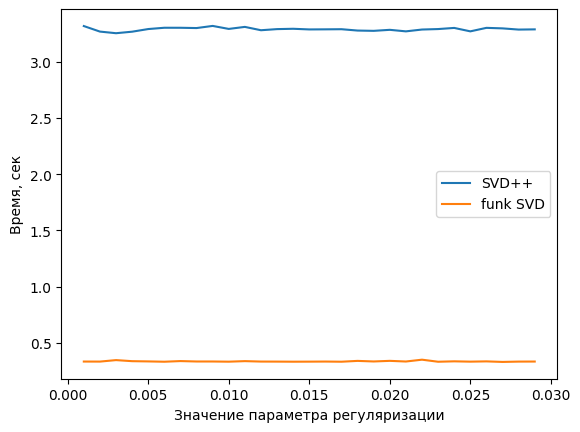
\includegraphics[width=\textwidth]{inc/timesReg.png}
	\caption{ График зависимости времени исполнения алгоритмов от значения параметра регуляризации.}
	\label{img:time1}
\end{figure}

\subsection{Зависимость времени исполнения алгоритмов от значения параметра скорости обучения}

На рисунке \ref{img:time2} представлен график зависимости времени исполнения алгоритмов от значения параметра скорости обучения.

\begin{figure}[H]
	\centering
	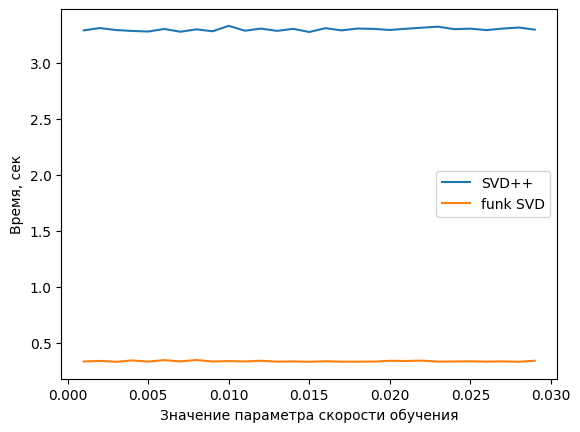
\includegraphics[width=\textwidth]{inc/timesLr.png}
	\caption{ График зависимости времени исполнения алгоритмов от значения параметра скорости обучения.}
	\label{img:time2}
\end{figure}

\subsection{Зависимость значения метрики RMSE алгоритмов от значения параметра регуляризации}

На рисунке \ref{img:time3} представлен график зависимости значения метрики RMSE от значения параметра регуляризации.

\begin{figure}[H]
	\centering
	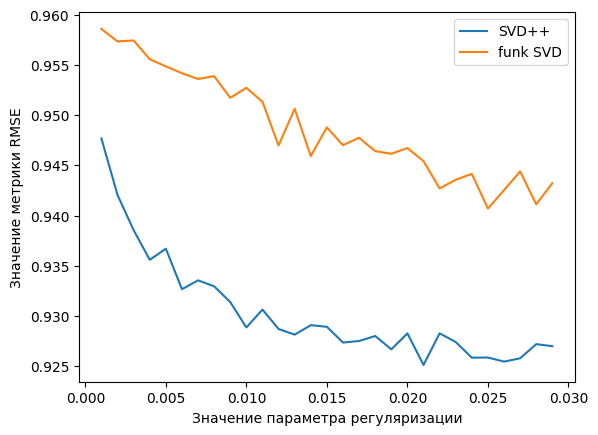
\includegraphics[width=\textwidth]{inc/rmseReg.png}
	\caption{ График зависимости значения метрики RMSE от значения параметра регуляризации.}
	\label{img:time3}
\end{figure}

\subsection{Зависимость значения метрики RMSE алгоритмов от значения параметра скорости обучения}

На рисунке \ref{img:time4} представлен график зависимости значения метрики RMSE от значения параметра скорости обучения.

\begin{figure}[H]
	\centering
	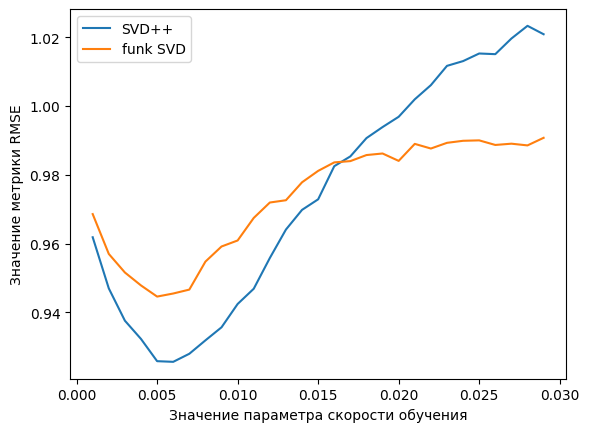
\includegraphics[width=\textwidth]{inc/rmseLr.png}
	\caption{ График зависимости значения метрики RMSE от значения параметра скорости обучения.}
	\label{img:time4}
\end{figure}

\subsection{Зависимость значения метрики MAE алгоритмов от значения параметра регуляризации}

На рисунке \ref{img:time5} представлен график зависимости значения метрики MAE от значения параметра регуляризации.

\begin{figure}[H]
	\centering
	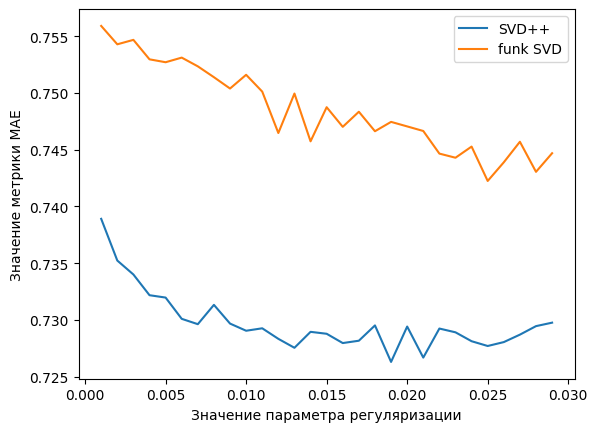
\includegraphics[width=\textwidth]{inc/maeReg.png}
	\caption{ График зависимости значения метрики MAE от значения параметра регуляризации.}
	\label{img:time5}
\end{figure}

\subsection{Зависимость значения метрики MAE алгоритмов от значения параметра скорости обучения}

На рисунке \ref{img:time6} представлен график зависимости значения метрики MAE от значения параметра скорости обучения.

\begin{figure}[H]
	\centering
	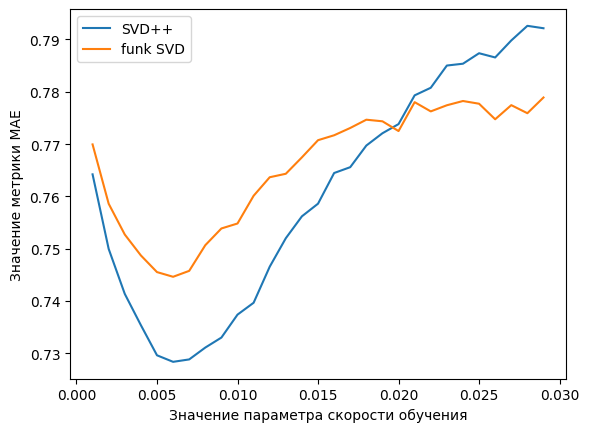
\includegraphics[width=\textwidth]{inc/maeLr.png}
	\caption{ График зависимости значения метрики MAE от значения параметра скорости обучения.}
	\label{img:time6}
\end{figure}

\subsection*{Заключение}

В результате проведенных исследований заметно, что SVD++ с включенным кэшированием на заданном датасете работает заметно медленнее, чем Funk SVD, как при изменении значения параметра регуляризации, так и при изменении значения параметра скорости обучения.

Также стоит отметить, что SVD++ при изменении параметра регуляризации показывает метрики RMSE и MAE меньше Funk SVD, однако при изменении параметра скорости обучения на значениях $\approx 0.16$ для RMSE и $\approx 0.20$ для MAE он начинает уступать по точности Funk SVD.